%For any $\omega$-category $\cat{C}$, the collection of natural functors $\cO(X) \to \cC$ is in bijection with that of cones under $\cO$ with apex $\cat{C}$.\anibal{Maybe there is more structure than just sets.}

%\subsection{Higher categories and Street orientals}
%



%We review the definition of $\omega$-category and of their underlying combinatorial structure, namely that of a globular set.
%
%\subsubsection{Globular sets}
%
%Recall that a directed graph consists of a set of edges $E$, a set of vertices $V$, and two functions $s,t \colon E \to V$, referred to as source and target.
%A globular set generalizes this notion including higher dimensional directed edges, which we refer to as cells.
%In precise terms, a \textit{globular set} $X$ is a diagram
%\[
%\begin{tikzcd}[column sep=15pt]
%	X_0 & \arrow[l,"\ s_0"',shift right=3pt] \arrow[l,"\ t_0",shift left=3pt] X_1
%	& \arrow[l,"\ s_1"',shift right=3pt] \arrow[l,"\ t_1",shift left=3pt] X_2
%	& \arrow[l,"\ s_2"',shift right=3pt] \arrow[l,"\ t_2",shift left=3pt] \dotsb
%\end{tikzcd}
%\]
%in the category of sets satisfying $s_{n-1}s_n = s_{n-1}t_n$ and $t_{n-1}s_n = t_{n-1}t_n$ for each $n \in \N_+$.
%Morphisms of globular sets are maps of diagrams.
%We refer to the elements in $X_n$ as \textit{$n$-cells} and define for $0 \leq k < n$ the \textit{$k$-source} and \textit{$k$-target maps} $s_k,t_k \colon X_n \to X_k$ as the unique maps that respectively factor through $s_k,t_k \colon X_{k+1} \to X_k$.
%Consult \cref{f:globes} for basic examples.
%
%The group $\rT^\infty := \Z_2^\mathbb{N}$ acts on the category of globular sets by permuting source and target maps.
%
%\begin{figure}
%	\begin{tikzpicture} [scale= .35]
	\draw node at (-4,0){ };
	\draw node at (4,0){ };
	\draw[fill] (-0.4,0) circle  [radius=3pt];

	\draw node at (-0.4,1){$n=0$} ;
	\draw node at (0,-2.4){} ;
\end{tikzpicture}
\begin{tikzpicture} [scale= .35]
	\draw[fill] (-4,0) circle  [radius=3pt];
	\draw[fill] (4,0) circle  [radius=3pt];

	\draw [->] (-4,0) [shorten >=0.2cm, shorten <=0.2cm,->] to (4,0) ;

	\draw node at (0,1){$n=1$} ;
	\draw node at (-6,-2.4){} ;
\end{tikzpicture}

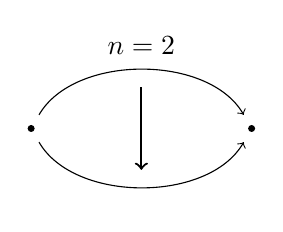
\begin{tikzpicture} [scale= .35]
	\draw[fill] (-4,0) circle  [radius=3pt];
	\draw[fill] (4,0) circle  [radius=3pt];

	\draw [->] (-4,0) [shorten >=0.2cm, shorten <=0.2cm,->, out=60,in=120] to (4,0) ;
	\draw [->] (-4,0) [shorten >=0.2cm, shorten <=0.2cm,->, out=-60,in=-120] to (4,0) ;

	\draw [->] (0,1.5) [thick] to (0,-1.5) ;

	\draw node at (0,3){$n=2$} ;
\end{tikzpicture}
\hspace*{25pt}
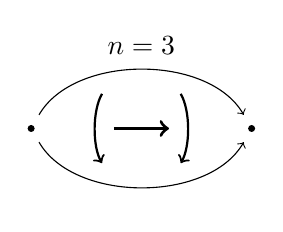
\begin{tikzpicture} [scale= .35]
	\draw[fill] (-4,0) circle  [radius=3pt];
	\draw[fill] (4,0) circle  [radius=3pt];

	\draw [->] (-4,0) [shorten >=0.2cm, shorten <=0.2cm,->, out=60,in=120] to (4,0) ;
	\draw [->] (-4,0) [shorten >=0.2cm, shorten <=0.2cm,->, out=-60,in=-120] to (4,0) ;

	\draw [->] (-1,2) [thick,shorten >=0.3cm, shorten <=0.3cm,->, out=-120,in=120] to (-1,-2) ;
	\draw [->] (1,2) [thick,shorten >=0.3cm, shorten <=0.3cm,->, out=-60,in=60] to (1,-2) ;

	\draw [->] (-1,0) [very thick] to (1,0) ;

	\draw node at (0,3){$n=3$} ;
\end{tikzpicture}
%	\caption{The $n$-globe $\bG^n$ for small values of $n$.}
%	\label{f:globes}
%\end{figure}
%
%\subsubsection{$\omega$-categories}
%
%Recall that a (small) category is a directed graph
%\[
%\begin{tikzcd}[column sep=15pt]
%	Ob & \arrow[l,"\ s_p"',shift right=3pt] \arrow[l,"\ t_p",shift left=3pt] Mor
%\end{tikzcd}
%\]
%with a partial composition satisfying associativity and unitality conditions.
%%\footnote{The adjective small is use to distinguish this notion from categories where objects or morphisms do not form sets.}
%An \textit{$\omega$-category} is a globular set $X$ with the structure of a category on
%\[
%\begin{tikzcd}[column sep=15pt]
%	X_p & \arrow[l,"\ s_p"',shift right=3pt] \arrow[l,"\ t_p",shift left=3pt] X_q
%\end{tikzcd}
%\]
%for each $p < q$ satisfying certain compatibility conditions for triples $p<q<r$.
%Morphisms of $\omega$-categories are morphisms of underlying globular sets preserving the compositional structure.
%We denote by $\wCat$ the category of $\omega$-categories.
%A complete definition can be found in \cite[\S1.2]{forest2022pasting}.
%The action of $\rT^\infty$ extends from globular sets to $\omega$-categories, and the automorphism associated to the $i^\th$ canonical tuple is referred to as the \textit{$i^\th$-opposite construction}.
%
%\subsection{$\omega$-diagrams}
%
%In this subsection we recall from \cite{steiner2004omega} the notion of \textit{augmented directed complex with a loop free basis}, which we shorten to \textit{$\omega$-diagram}, and the fully faithful functor from the category of these to that of $\omega$-categories.
%See \cite[\S1.6]{forest2022pasting} for another presentation of these ideas.
%
%\subsubsection{Cells}
%
%Let $C$ be a based chain complex, i.e. a chain complex of free abelian groups together with a chosen basis.
%Denote the natural augmentation map by $\aug: C \to \Z$.
%We will naturally assign a globular set $\cells(C)$ to $C$ as follows.
%An $n$-cell in $\cells(C)$ is an $(2n+1)$-tuple
%\[
%(c_0^-,c_0^+,\dots,c_{n-1}^-,c_{n-1}^+,c_n)
%\]
%with each entry a positive element in $C$ satisfying:
%\begin{enumerate}
%	\item $\bd(c_k^\pm) = c_{k-1}^+ - c_{k-1}^-$ for $k \in \set{1,\dots,n-1}$,
%	\item $\bd c_n = c_{n-1}^+ - c_{n-1}^-$ if $n > 0$,
%	\item $\aug(c_0^-) = \aug(c_0^+) = 1$.
%\end{enumerate}
%Its source and target maps are given by
%\begin{align*}
%	&s_{n-1}(c_0^-, \dots, c_{n-1}^+, c) =
%	(c_0^-, \dots, c_{n-2}^+, c_{n-1}^-), \\
%	&t_{n-1}(c_0^-, \dots, c_{n-1}^+, c) =
%	(c_0^-, \dots, c_{n-2}^+, c_{n-1}^+).
%\end{align*}
%
%\subsubsection{Basic cells}
%
%Let $b \in C_n$ be a basis element, its \textit{basic cell} $\angles{b} \in \cells(C)$, referred to as \textit{atom} by Steiner, is the $n$-cell
%\[
%(\angles{b}_0^-,\angles{b}_0^+,\dots,\angles{b}_{n-1}^-,\angles{b}_{n-1}^+,\angles{b}_n)
%\]
%with $\angles{b}_n = b$ and, for $\varepsilon \in \{-,+\}$,
%\[
%\angles{b}_k^\varepsilon =
%\begin{cases}
%	\bd^\varepsilon b & k = n-1, \\
%	\bd^\varepsilon \angles{b}^\varepsilon_{k+1} & k < n-1.
%\end{cases}
%\]
%
%For two basis elements of degree greater than $k$ we write $b <_k b'$ if the same basis element appears with a nonzero coefficient in both $\angles{b}^+_k$ and $\angles{b'}^-_k$.
%
%\subsubsection{$\omega$-diagrams}
%
%\begin{definition}
%	\label{def:chain-loop-free}
%	An \textit{$\omega$-diagram} is a based chain complex satisfying:
%	\begin{enumerate}
	%		\item\label{i:loop-free} For each $k$, the transitive closure of the relation $<_k$ is irreflexive.
	%		\item\label{i:unital} For each $\varepsilon \in \set{-,+}$ and basis element $b$,
	%		\[
	%		\aug\, \angles{b}^\varepsilon_0 = 1.
	%		\]
	%	\end{enumerate}
%	We we will refer to these as the \textit{loop-free} and \textit{unital} conditions respectively.
%\end{definition}
%
%For an $\omega$-diagram $C$, all entries in the cells of $\cells(C)$ are sums of basis elements, not just positive elements \cite[Theorem 4.1]{steiner2012opetopes}.
%
%We denote the category of $\omega$-diagrams with positive augmentation-preserving chain maps by $\wDiag$.
%The group $\rT^\infty$ acts on $\wDiag$ by acting on the underlying chain complex.
%
%\subsection{From $\omega$-diagrams to $\omega$-categories}\label{ss:free omega-category}
%
%Let $C$ be an $\omega$-diagram.
%The globular set $\cells(C)$ can be given a natural $\omega$-category structure with
%identities defined by
%\[
%\id(c_0^-, \dots, c_{n-1}^+, c) = (c_0^-, \dots, c_{n-1}^+, c, c, 0),
%\]
%and $i$-compositions by
%\begin{multline*}
%	(d_0^-, \dots, d_{n-1}^+, d) \circ_i (c_0^-, \dots, c_{n-1}^+, c) = \\
%	(c_0^-, \dots, c_{i-1}^+, c_i^-, d_i^-,  c_{i+1}^- + d_{i+1}^-, \dots, c_{n-1}^- + d_{n-1}^-, c+d).
%\end{multline*}
%This assignment defines a $\rT^\infty$-equivariant fully faithful functor
%\[
%\nu \colon \wDiag \to \wCat.
%\]
%Furthermore, $\nu(C)$ is freely generated by the basic cells of $\cells(C)$.
%We refer to the original reference \cite{steiner2004omega} or to the more general discussion of freeness presented in \cite{forest2022pasting} for more details.
%
%\subsection{Street orientals}\label{ss:orientals}
%
%Let $\chains(\gsimplex^n)$ be the usual based chain complex of the standard $n$-simplex.
%Explicitly, its basis of degree $k$ elements consists of tuples $[v_0,\dots,v_k]$ of distinct integers in $\{0,\dots,n\}$, with boundary defined by
%\[
%\bd\, [v_0,\dots,v_k] = \sum_{i=0}^k (-1)^i [v_0,\dots,\widehat{v}_i,\dots,v_k].
%\]
%Please refer to \cite[Example 3.8]{steiner2004omega} for the verification that this based chain complex satisfies the loop-free and unital conditions.
%Examples of atoms associated with this $\omega$-diagram are provided in \cref{f:street}.
%As demonstrated by Steiner in the same reference, the free $\omega$-category defined by this $\omega$-diagram is isomorphic to the oriental $\oriental_n$ introduced by Street in \cite{street1987orientals}.
%
%\begin{figure}
%	\centering
%	\begin{small}
	\begin{verbatim}
		[0,] | [1,]
		---------------
		[0,] | [2,]
		[0,2] | [0,1] + [1,2]
		---------------
		[0,] | [3,]
		[0,3] | [0,1] + [1,2] + [2,3]
		[0,2,3] + [0,1,2] | [0,1,3] + [1,2,3]
		---------------
		[0,] | [4,]
		[0,4] | [0,1] + [1,2] + [2,3] + [3,4]
		[0,3,4] + [0,2,3] + [0,1,2] | [0,1,4] + [1,2,4] + [2,3,4]
		[0,2,3,4] + [0,1,2,4] | [0,1,2,3] + [0,1,3,4] + [1,2,3,4]
	\end{verbatim}
\end{small}
%	\caption{The atom of the top degree basis element of $\chains(\gsimplex^n)$ for $n \in \{1,2,3,4\}$ obtained using \href{https://github.com/ammedmar/wcat}{\texttt{wcat}}.}
%	\label{f:street}
%\end{figure}

%\subsection{$\omega$-categories}
%
%We will consider $n$-\textit{categories} recursively defined as categories enriched in $(n-1)$-categories.
%We will take the one-sorted viewpoint identifying an $n$-category $\cC$ with a set $\Mor\cC$ together with, for $i = 0,\dots n-1$, \textit{source} and \textit{target functions}
%\[
%s_i, t_i \colon \Mor\cC \to \Mor\cC
%\]
%and \textit{partial compositions}
%\[
%\circ_i \colon \Mor\cC \times \Mor\cC \to \Mor\cC
%\]
%with $a \circ_i b$ defined when $s_i a = t_i b$.
%For a complete list of relations satisfied by these please consult \cite[Definition 2.1]{steiner2004omega}.
%An $n$-category is naturally a $(n+1)$-category, and we define $\omega$-category as the limiting notion.
%
%We now will describe $\omega$-categories defined freely from combinatorial data, generalizing the construction of $1$-categories from directed graphs.
%
%\subsection{Pasting schemes}
%
%Let $C$ be a chain complex with a basis $B$.
%For any $c \in C$, writing $\bd\, c$ in the basis, we define $\bd^\varepsilon c$ for $\varepsilon \in \{+,-\}$ by the equation
%\[
%\bd\, c = \bd^+c - \bd^-c.
%\]
%For any $\varepsilon \in \{+,-\}$ and basis element $b$ define its \textit{atom} recursively by
%\[
%\angles{b}^\varepsilon_k =
%\begin{cases}
%	0 & \bars{b} > k, \\
%	b & \bars{b} = k, \\
%	\bd^\varepsilon \angles{b}^\varepsilon_{k+1} & \bars{b} < k.
%\end{cases}
%\]
%For two basis elements of degree greater than $k$ we write $a <_k b$ if there is a basis element with a nonzero coefficient in both $\angles{a}^+_k$ and $\angles{b}^-_k$.
%
%\begin{definition*}
%	A \textit{pasting scheme} is a chain complex with a basis $B$ such that:
%	\begin{enumerate}
	%		\item\label{i:loop-free} For each $k$, the relation $<_k$ makes $B$ into a poset.
	%		\item\label{i:unital} For each $b \in B$ and $\varepsilon \in \{+,-\}$, the element $\angles{b}^\varepsilon_0$ is equal to a basis element.
	%	\end{enumerate}
%	We we will refer to these as the \textit{loop-free} and \textit{unital} conditions respectively.
%\end{definition*}
%
%We will mostly concern ourselves with the notion of pasting scheme as defined above.
%But, for completeness, we will review in the next two subsections their freely generated $\omega$-categories.
%
%\subsection{Free $\omega$-categories}
%
%The starting point of Steiner's construction is a form of Dold--Kan correspondence appearing in work by R. Brown and P. J. Higgins \cite{brown1981cubes}.
%They show that (non-negatively graded) chain complexes are equivalent to $\omega$-category objects in the category of abelian groups using a functor we now described on objects.
%Given a chain complex $C$, we consider all elements
%\[
%c = (c_0^-,c_0^+,c_1^-,c_1^+,\dots)
%\]
%in the infinite product of $C$ with itself satisfying the following conditions for all $k \in \N$ and $\varepsilon \in \{-,+\}$:
%\begin{enumerate}
%	\item $c_k^\varepsilon \in C_k$,
%	\item $c_k^\varepsilon \neq 0$ except for finitely many $k$,
%	\item $\bd c_{k+1}^\varepsilon = c_k^+ - c_k^-$.
%\end{enumerate}
%We now describe for each $k \in \N$, its source and target functions
%\begin{align*}
%	&s_k(c) = (c_0^-,c_0^+,\dots,c_{k-1}^-,c_{k-1}^+,c_k^-,c_k^-,0,0,\dots),\\
%	&t_k(c) = (c_0^-,c_0^+,\dots,c_{k-1}^-,c_{k-1}^+,c_k^+,c_k^+,0,0,\dots),
%\end{align*}
%and partial composition
%\[
%c \circ_k c' = c+c'-c'',
%\]
%where $t_k(c) = s_k(c') = c''$.
%
%Steiner defines the $\omega$-category freely generated by a pasting scheme by considering the $\omega$-category generated by the atoms of the pasting scheme inside this abelian $\omega$-category.
%
%\subsection{Street's orientals}\label{ss:orientals}
%
%Let $\gchains(\gsimplex^n)$ be the usual chain complex of the standard $n$-simplex.
%Explicitly, its basis of degree $k$ elements consists of tuples $[v_0,\dots,v_k]$ of distinct integers in $\{0,\dots,n\}$, with boundary defined by
%\[
%\bd\, [v_0,\dots,v_k] = \sum_{i=0}^k (-1)^i [v_0,\dots,\widehat{v}_i,\dots,v_k].
%\]
%To verify that this based chain complex satisfies the loop-free and unital conditions, please refer to \cite[Example 3.8]{steiner2004omega}.
%Examples of atoms associated with this pasting scheme are provided in \cref{f:street}.
%As demonstrated by Steiner in the same reference, this pasting scheme defines a free $\omega$-category that is isomorphic to the Street oriental $\cO_n$ \cite{street1987orientals}.
%
%\begin{figure}
%	\centering
%	\begin{small}
	\begin{verbatim}
		[0,] | [1,]
		---------------
		[0,] | [2,]
		[0,2] | [0,1] + [1,2]
		---------------
		[0,] | [3,]
		[0,3] | [0,1] + [1,2] + [2,3]
		[0,2,3] + [0,1,2] | [0,1,3] + [1,2,3]
		---------------
		[0,] | [4,]
		[0,4] | [0,1] + [1,2] + [2,3] + [3,4]
		[0,3,4] + [0,2,3] + [0,1,2] | [0,1,4] + [1,2,4] + [2,3,4]
		[0,2,3,4] + [0,1,2,4] | [0,1,2,3] + [0,1,3,4] + [1,2,3,4]
	\end{verbatim}
\end{small}
%	\caption{The (non-trivial part of the) atom of the top dimensional basis element in $\gchains(\gsimplex^n)$ for $n \in \{1,2,3,4\}$. (Computations done using \href{https://github.com/ammedmar/wcat}{\texttt{wcat}}.)}
%	\label{f:street}
%\end{figure}